\documentclass[paper=a4, fontsize=11pt]{scrartcl}
\usepackage[letterpaper, margin=0.85in]{geometry}
\usepackage[T1]{fontenc}
\usepackage{fourier}
\usepackage{ragged2e}

\usepackage[english]{babel}															
\usepackage[protrusion=true,expansion=true]{microtype}	
\usepackage{amsmath,amsfonts,amsthm} 
\usepackage[pdftex]{graphicx}	
\usepackage{url}


\usepackage{sectsty}
\allsectionsfont{\centering \normalfont\scshape}

% Libraries added by Kyle
\usepackage[parfill]{parskip} % Skip in between paragraphs instead of indenting
\usepackage{wrapfig} % Figures to the side of text / text wrapping around figures
\usepackage{caption} % Captioning of figures
\usepackage{fancyref} % Referencing of figures and updates automatically as figures change number
\usepackage{float}
\usepackage[table]{xcolor}
\setlength\parindent{0pt}
% End libraries added by Kyle

\usepackage{fancyhdr}
\pagestyle{fancyplain}
\fancyhead{}											
\fancyfoot[L]{}											
\fancyfoot[C]{}											
\fancyfoot[C]{\thepage}									
\renewcommand{\headrulewidth}{0pt}			
\renewcommand{\footrulewidth}{0pt}				
\setlength{\headheight}{13.6pt}


\numberwithin{equation}{section}		
\numberwithin{figure}{section}			
\numberwithin{table}{section}				


\newcommand{\horrule}[1]{\rule{\linewidth}{#1}} 

\title{
		%\vspace{-1in} 	
		\usefont{OT1}{bch}{b}{n}
		\normalfont \normalsize \textsc{University of California, Los Angeles} \\ [25pt]
		\horrule{0.5pt} \\[0.4cm]
		\huge Cry, Cry, Cry \\
		\horrule{2pt} \\[0.5cm]
}
\author{
		\normalfont \normalsize Kyle Colton \\
        \normalfont \normalsize Christian Gao \\
        \normalfont \normalsize  Benjamin Hong \\
        \normalfont \normalsize Feiran Zhu\\
}
\date{}


\begin{document}
\maketitle


\includegraphics[width=\textwidth]{baby.jpg}
\newpage

\tableofcontents
\newpage
\noindent \horrule{0.5pt} 
{\textbf{\\ Objective.}}
The purpose of this study is to discuss algorithms designed to predict whether or not a baby is crying. 
{\textbf{\\ Data Collection and Procedure.}}
We were given a multitude of audio files (in WAV format) of animal, baby, and adult sounds. We analyzed the pitch of each sound using two different procedures: (1) using FOSS \textit{aubio} and conducting K-means clustering, which is an iterative classification method that we will discuss in more detail later, and support vector machine (SVM) classification and (2) using a specially designed pitch extraction algorithm to ultimately use the Baum-Welch algorithm to answer a number of questions that we will make clear throughout the report.
{\textbf{\\ Conclusion.}}
We arrived at a decent classification algorithm using K-means and SVM, but because of limitations in the data, we did not end up with an extremely successful algorithm based on HMM.  \\
\horrule{0.5pt} \\[0.4cm]
% * <bendhong@ucla.edu> 2015-06-06T23:36:04.154Z:
%
% 
%
% * <bendhong@ucla.edu> 2015-06-06T23:36:05.493Z:
%
% 
%
\section{Abstract}
% * <bendhong@ucla.edu> 2015-06-06T23:36:06.752Z:
%
% 
%
Caring for a baby requires patience and effective communication. A caretaker attends to the baby when he/she cries, but this strictly involves an auditory process. We can see how this becomes problematic for parents who are deaf or have difficulty hearing. Fortunately, because of technological advances, there are now devices that assist parents in determining whether or not their child is crying. Of course, for a device to accurately decipher noises, the algorithm must be able to distinguish between different noises (e.g., between a dog crying and a baby crying). This report discusses the algorithms we designed to predict the baby's emotional state---that is, is the baby crying, laughing, or neutral? 


\section{Questions}
\begin{enumerate}
	\item Can we design an algorithm that accurately predicts whether or not a baby is crying?
	\item Given that our algorithm works, what is its prediction rate---that is, how often does our algorithm successfully classify noises into their respective categories?
\end{enumerate}

%\section{Variable Description}
%
%Essentially, we were only considered with one variable, \textbf{PITCH}, which we divided into four levels: high pitch, medium pitch, low pitch, and no pitch.

\section{Description of Data}
For this project, we were given 183 \texttt{wav} files split between several sounds:
\begin{center}
\begin{tabular}{r l}
19 & Adult Female Cry\\
15 & Adult Female Laugh \\
15 & Adult Male Laugh \\
15 & Adult Female Neutral \\
15 & Adult Male Neutral \\
15 & Animal Cat\\
15 & Animal Dog\\
21 & Baby Cry \\
18 & Baby Laugh \\
25 & Baby Neutral
\end{tabular}
\end{center}
Each file is approximately 1.5 seconds in length and contains lossless sound without background noise. Each file is labeled according to the contents. 
\section{Classification using Pitch Analysis}
Pitch detection and analysis was explored as a method to identify baby cries. The detection method relies on the assumption that pitch patterns for each sound type will differ, but within the sound types each sample will be similar.

\begin{wrapfigure}{r}{.4\textwidth}
\begin{center}
\vspace{-20pt}
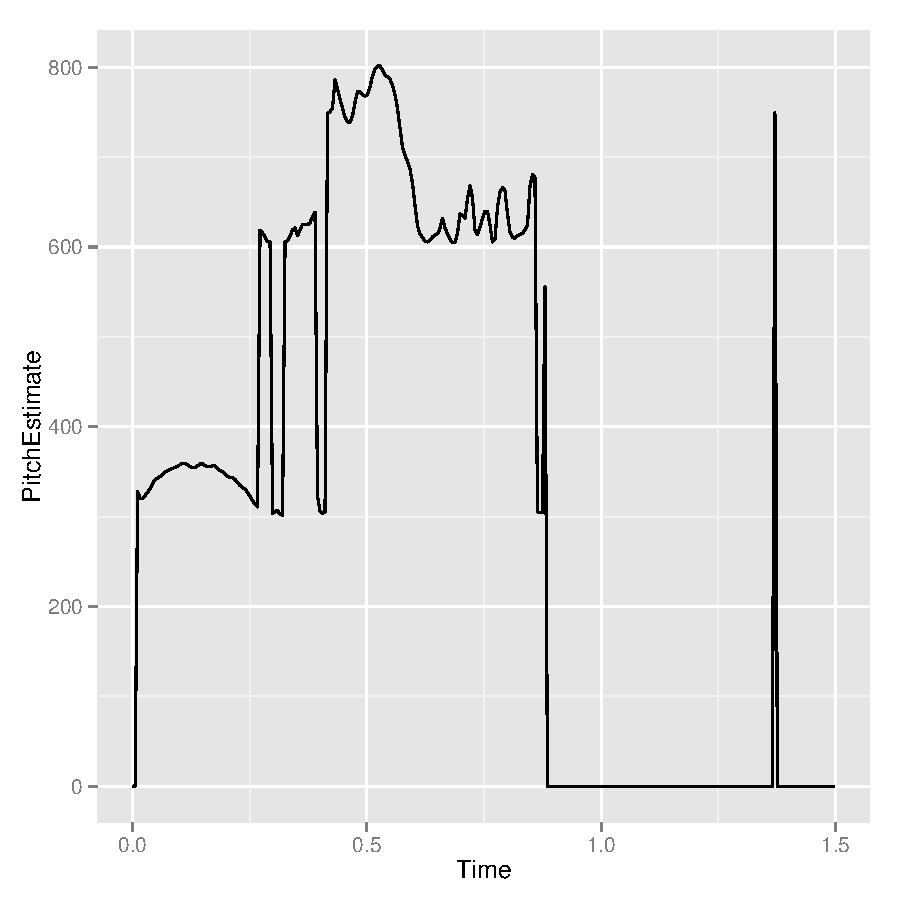
\includegraphics[width=.38\textwidth]{pitch_time.pdf}
\caption{Pitch estimate of a \texttt{wav} file}\label{fig:aubiograph}
\vspace{-20pt}
\end{center}
\end{wrapfigure}

Raw audio files (stored as \texttt{wav}) were run through a Free/Libre and Open Source Software package called Aubio\footnote{Package information can be found at \url{aubio.org} or at \url{http://git.aubio.org}}. Aubio is a C-based audio labeling tool that includes several methods and controllable methods for pitch detection in an audio stream.

In order to complete pitch analysis, each 1.5 second \texttt{wav} file was fed through Aubio to get time-series pitch data, then broken into ``events'' based on silence. In figure \ref{fig:aubiograph}, we see an estimate of pitches over time for one such file. This file, for example would be broken into two events. The main event stretches from approximately $t=0.00$ to $t=0.85$. A second event occurs around $t=1.40$.

Looking at the graph, it appears that the second event in this file is an error. It is a blip caused by something in the recording that we can safely ignore if we can identify it and separate it from the good data. An easy approximation is to ignore all events shorter than a set time interval. After testing all time intervals using a given model, $t=0.1$ seconds was chosen as the cutoff for ``real'' versus ``fake'' events.

\begin{wrapfigure}{l}{.3\textwidth}
\begin{center}
\vspace{-15pt}
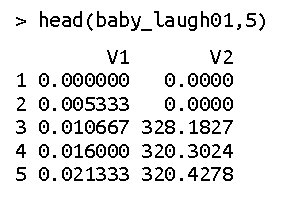
\includegraphics[width=.28\textwidth]{aubio_out.pdf}
\caption{Data from Aubio with time (l) and pitch (r)}\label{fig:headaubio}
\end{center}
\vspace{-20pt}
\end{wrapfigure}

After events were detected and pre-processed, summary statistics were collected on each event. Each event was stored with filename, event type (baby\_cry, baby\_laugh, etc.), minimum pitch, 1st quartile, median pitch, 3rd quartile, maximum pitch, mean pitch, and length of the event. Models were then run on these summary statistics to capture and classify them and compare them to the originating source. To start with, the models were built around using the events individually. Eventually, smarter models were built to consider all events from a single file as a unit and decide by voting on the predicted classification of those files.

\begin{figure}[H]
\begin{center}
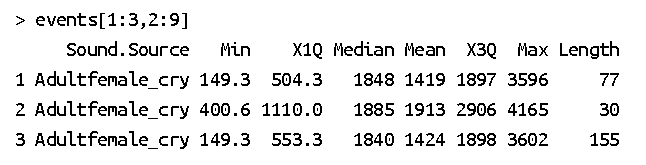
\includegraphics[width=.65\textwidth]{aubio_events.pdf}
\caption{Summary statistics produced from the Aubio output}
\end{center}
\end{figure}

\subsection{Measuring Results}

A baby detector, by nature, is attempting to find when the baby is unhappy by listening for crying. With this in mind, the power of the model (the correct identification of an event when one occurs) is far more important than any other statistics\footnote{This is true within reason; we don't want parents to become complacent because of too many false positives}. For this reason, the models assume that if one event is categorized as a \texttt{baby\_cry} event, then that file is a \texttt{baby\_cry} event. This increases power at the expense of accuracy.

Additionally, the model was simplified into a binary outcome of a baby crying or not crying. While model was able to classify with some success the other events, the purpose of the monitor is to detect a baby crying, so the model was simplified.

\begin{center}
\begin{tabular}{ r | c | c |}
Total Population & Baby is Crying & Baby is not Crying \\\hline
Predicted Crying & \cellcolor{green!25}True Positive (TP) & \cellcolor{red!25}False Positive (FP) \\\hline
Predicted Not Crying & \cellcolor{red!25}False Negative (FN) & \cellcolor{green!25}True Negative (TN)\\\hline
\end{tabular}
\end{center}

The false positive (FP) is also referred to as Type 1 Error. Similarly, the false negative is referred to as Type 2 Error. The main statistics explored for ranking models were:\\
\begin{itemize}
\item Overall prediction rate (or accuracy):
\begin{align*}
ACC = \frac{\sum TP + \sum TN}{\sum \text{Total Population}}
\end{align*}
\item Power (also known as Sensitivity or True Positive Rate (TPR)):
\begin{align*}
TPR = \frac{\sum TP}{\sum TP + \sum FN}
\end{align*}
\item Precision (also known as the Positive Predictive Value (PPV)):
\begin{align*}
PPV = \frac{\sum TP}{\sum TP + \sum FP}
\end{align*}
\end{itemize}

In simple terms, the accuracy is the fraction of total stuff that was correctly classified. Power is the number of times we caught the baby crying over the number of times it did cry. Precision is the fraction of times we thought the baby was crying where the baby was actually crying.

\subsection{K-Means Applied to Pitch Estimates}
K-means was selected as a candidate classification model because of its relative simplicity. K-means uses euclidean distance between each of the vectors to classify the data into $k$ groups of the shortest distance. The groups are then used to remap the centroids to the mean of each group, and the groups are calculated again. This process continues until an update causes no change in the group assignments, at which point the model has converged.

\subsubsection{Performance of K-Means}\label{subsubsec:LOOCV}
The model was checked using Leave One Out Cross Validation (LOOCV). All but one \texttt{wav} files were used in the model. The result was predicted on the left-out \texttt{wav} file. This process was repeated until every file had been left out and the subsequently tested against. Because multiple events may exist per file, several were included in each validation of the model.

While the overall prediction rate of k-means grew over time, the power decayed. The best option for a value of k is therefore $k=2$. However, the performance at $k=1$ suggests that there is not a very clear-cut grouping to choose. Therefore, we should expect that a more complex model may perform better. K-means is a fast algorithm and is easy to understand, but the reliance on euclidean distances hampers the performance.

\begin{figure}[H]
\begin{center}
\vspace{-100pt}
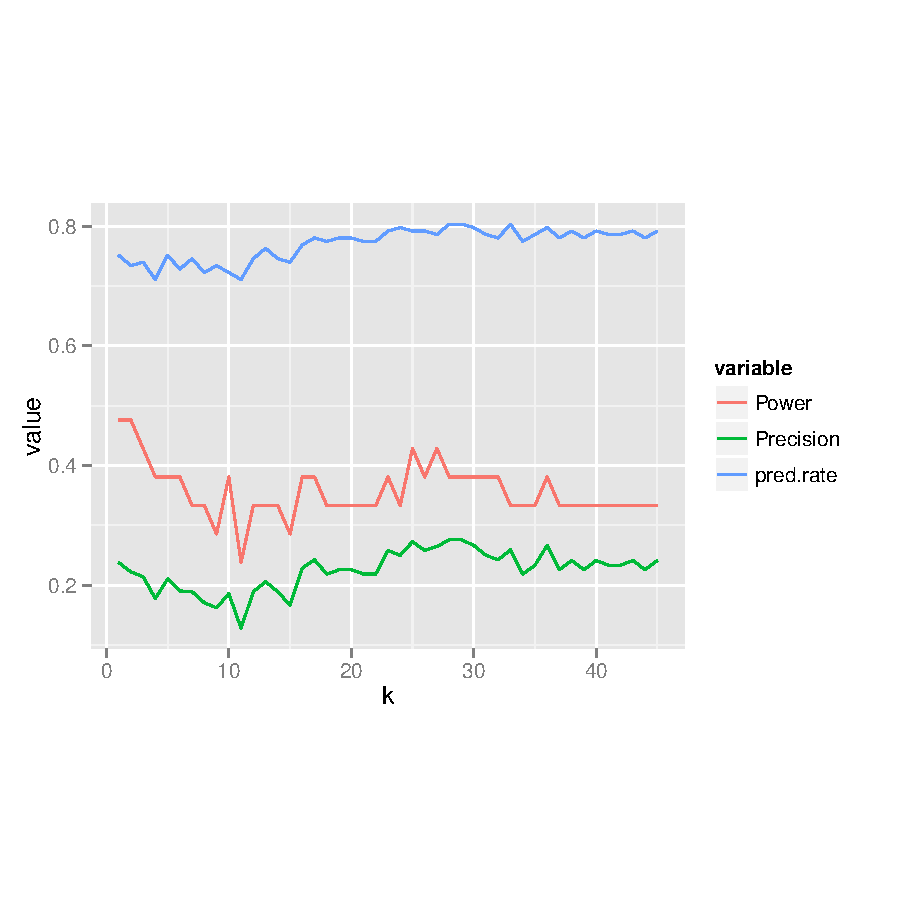
\includegraphics[width=\textwidth]{k_means.pdf}
\vspace{-120pt}
\caption{Performance K-means for various values of $k$}
\end{center}
\end{figure}

\subsection{Support Vector Machine Applied to Pitch Estimates}
A Support Vector Machine (SVM) is a machine learning supervised model that attempts to separate classes of data using a training set and a given method. SVM is able to perform non-linear classification by using multidimensional planes and shapes and so may be more suited to the classification task than K-means.

\noindent SVM relies on a set kernel and cost for solving a model. The kernel dictates what hyperplanes SVM can and will use in it's modeling. In soft SVM, the cost variable dictates the ``cost'' or punishment of the model for violating the classifications during the training phase. Alternatively, hard SVM will fail to missclassify, but may also fail to converge for that reason. This data was not linearly separable, so SVM was unable to sort the sounds exactly, but a reasonable hyperplane was drawn.

\noindent The SVM model was run in \texttt{R} using the \texttt{e1071} package\footnote{\url{http://cran.r-project.org/web/packages/e1071/e1071.pdf}}.

\subsubsection{Performance of SVM}
The model was checked using LOOCV in the same style as was done for K-means (see \ref{subsubsec:LOOCV} for details). Multiple tests were performed with various kernels (sigmoid, polynomial and linear), but the radial basis kernel was found to perform the best. Using the radial basis kernel, we varied the misclassification cost and ran the model, producing a plot of Power and Accuracy at various costs.

Power initially starts very low, but rises as cost increases to approximately $cost = 25$. Once we maximize power, the best prediction rate appears at around $cost = 27$.

\begin{figure}[H]
\begin{center}
\vspace{-100pt}
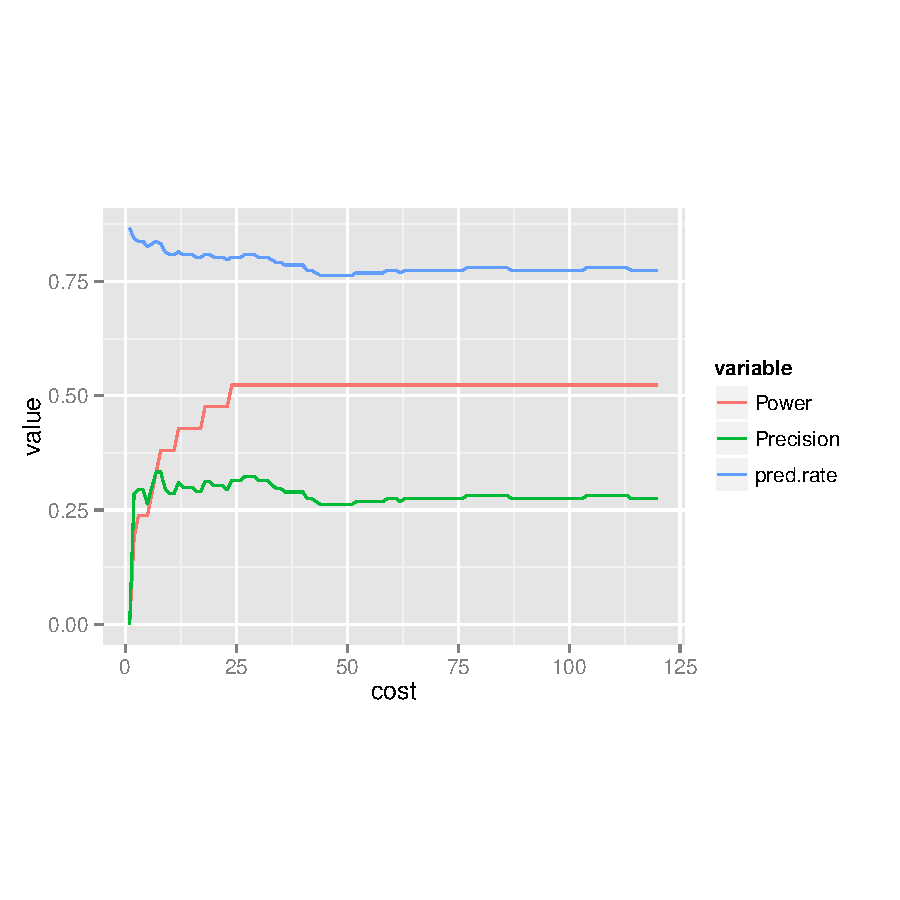
\includegraphics[width=\textwidth]{svm_accuracy.pdf}
\vspace{-120pt}
\caption{Performance of SVM versus misclassification cost}
\end{center}
\end{figure}

\subsection{Comparison of K-Means and SVM}
In this experiment, we saw slight benefits in using SVM over K-Means. Using 2 clusters, K-Means achieved a prediction rate of approximately $ACC = 0.734$, a power of $TPR = 0.476$, and a precision of $PPV = 0.222$. At $cost = 27$, SVM saw a prediction rate of $ACC = 0.809$, a power of $TPR = 0.524$, and a precision of $PPV = 0.324$. SVM was able to correctly classify more often, and achieve a higher power, catching slightly over half of all the baby cries.

While K-Means has likely reached its limits with this Data, we would expect SVM to continue to improve given more data. Unfortunately, SVM is generally very computationally expensive compared to K-Means. With the increased complexity, though comes better modeling capabilities.

\subsection{Future Improvements}
Improvements can be made by including other measurement points, for example, relative volume. We would expect, for example that a baby crying and a baby laughing would have distinctly different volumes. Combining both volume and pitch analysis would likely improve the model.

Additionally, we could expect that given a larger dataset, the classification would improve. This is especially true if SVM is allowed to train on a particular baby's sounds.

\section{Hidden Markov Model} 

\begin{center}
\textbf{Old Transition Matrix}

\begin{tabular}{ |c|c|c|c| } 
 \hline
       & Cry & Neutral & Laugh \\
 \hline
 Cry & 0.8 & 0.15 & 0.05 \\ 
 Neutral & 0.2 & 0.6 & 0.2 \\ 
 Laugh & 0.05 & 0.35 & 0.6 \\
 \hline
\end{tabular}

\begin{huge}$\downarrow$\end{huge}

\textbf{New Transition Matrix}

\begin{tabular}{ |c|c|c|c| } 
 \hline
       & Cry & Neutral & Laugh \\
 \hline
 Cry & 0.85 & 0.1 & 0.05 \\ 
 Neutral & 0.15 & 0.7 & 0.15 \\ 
 Laugh & 0.1 & 0.4 & 0.5 \\
 \hline
\end{tabular}
\end{center}

%\begin{wrapfigure}{l}{.25\textwidth}
%\begin{center}
%\vspace{-15pt}
%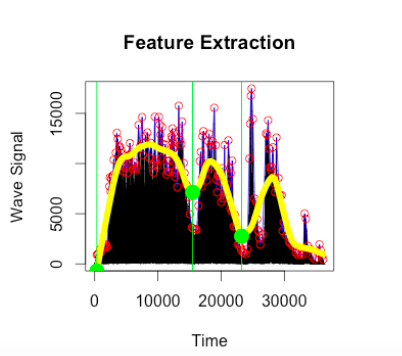
\includegraphics[width=.25\textwidth]{plot.png}
%\end{center}
%\vspace{-20pt}
%\end{wrapfigure}

The third approach we tried is to apply Hidden Markov Model to our crying baby data in order to get simulated prediction results. As we decided to use pitch as the predictor and classified it into four categories--high pitch, medium pitch, low pitch, and no pitch, we first need to extract pitches from the WAV file. We designed an algorithm to get the maximum pitch at every point in time, smooth the max points into an envelope pitch curve, and separate the max pitch curve at the troughs. The resulted separation plot is shown. The second step was to get parameters for the Hidden Markov Model. We got the emission matrix directly by summarizing the original data. For the transition matrix, however, we did not have a reliable basis and had to arbitrarily make the transition probability of crying to laughing or to making neutral sounds. Then we applied Viterbi algorithm to find the most likely combinations in the sequence of pitches we extracted.

\subsection{Using Baum-Welch Algorithm}

Our simulated results shows an around 40\% percent success rate of determining whether the baby is crying or laughing. Honestly, this success rate is not compelling due to the many constraints in our data and model which are discussed in \ref{subsec:hmmshort}.

%\section{Conclusion}
%Ultimately, we ended up with three models, two of which performed fairly well (K-means and SVM), and one that given a more comprehensive dataset may yield better results.

\subsection{Shortcomings}\label{subsec:hmmshort}
We encountered many problems when applying the Hidden Markov Model in the prediction. The small sample size led us to one of our first problems. Since we only have 62 WAV files related to baby sounds, we could not get a reliable estimation for the initial emission matrix used in the hidden Markov model. Given the fact that the accuracy of hidden Markov model heavily relies on the emission matrix and transition matrix, the lack of a reliable emission matrix compromises our success rate. That the length of each audio recorded is really short was also problematic for us. Most of the recorded sounds are less than 2 seconds. It is relatively hard to determine whether a baby is crying or laughing with just one sound lasting for only one second. If we could get a substantially large sample with each recording lasting for more than one hour, we are confident that our simulated results would be much more reliable. Another shortcoming of our model is that we could not get a convincing transition matrix. The transition matrix lists the probability that a cry sound would stay crying, or change to either laugh or neutral in the next state. We arbitrarily determined the transition probabilities in our model, and this matrix might be significantly different from the real transition probabilities.

\subsection{Recommendations}
Though the algorithm based on the hidden Markov model only performed slightly better than a random number generator, we believe that with a more comprehensive data set, we would be able to yield more appealing results. Ideally, the data set would consist of hours and hours of long recordings of baby noise and have over 10,000 observations of individual baby noises. With such a data set in hand, we would be able to answer the following questions (and therefore conduct a more thorough analysis using HMM):

\begin{itemize}
	\item What is the probability that a baby will cry right after laughing?
    \item When does the baby usually sleep?
    \item What is the probability that a baby cries right after waking up?
    \item What is the average time that a baby cries, laughs and is neutral? 
\end{itemize}

\end{document}
